\chapter{Analisis}
\label{chap:analisis}

Untuk menyelesaikan masalah pengelompokan dokumen menggunakan algoritma genetika, maka perlu dibangun sebuah model yang dapat diterapkan ke dalam algoritma tersebut.

\section{Representasi Kromosom}
Setiap \textit{string} kromosom merupakan deretan bilangan riil yang merepresentasikan $K$ titik pusat \textit{cluster} (\textit{centroid}). Dalam ruang $N$ dimensi, panjang dari kromosom akan menjadi $N\times K$ gen. $N$ kata pertama merepresentasikan $N$ dimensi dari \textit{centroid} pertama, $N$ kata selanjutnya merepresentasikan $N$ dimensi dari \textit{centroid} kedua, dan seterusnya.

\section{Fungsi \textit{Fitness}}
Perhitungan \textit{fitness} dalam penelitian ini terdiri dari dua tahap. Pada tahap pertama, terjadi pembentukan \textit{cluster} berdasarkan titik pusat yang terkandung dalam kromosom. Hal ini dilakukan dengan menetapkan setiap titik $x_i,i=1,2, ... ,n$ ke dalam sebuah \textit{cluster} $C_j$ dengan \textit{centroid} $z_j$ sehingga

\begin{equation}
\Vert x_i-z_j \Vert < \Vert x_i-z_p \Vert , p=1,2, ... ,K \mbox{, dan } p \neq j.
\end{equation}

Setelah proses pengelompokan selesai, titik pusat yang terkandung dalam kromosom diganti dengan rata-rata titik dari tiap \textit{cluster}. Dengan kata lain, untuk \textit{cluster} $C_i$, \textit{centroid} baru $z_i^*$ dapat dihitung dengan rumus:

\begin{equation}
z_i^*=\frac{1}{n_i} \sum_{x_j\in C_i} x_j,   i=1,2, ... ,K.
\end{equation}

dengan $z_i^*$ merupakan titik pusat \textit{cluster} ke-$i$, $n_i$ merupakan jumlah anggota \textit{cluster} ke-$i$, dan $x_j$ merupakan titik ke-$j$ yang merupakan anggota dari \textit{cluster} ke-$i$. $z_i^*$ ini akan menggantikan $z_i$ sebelumnya di kromosom. Ada dua metode perhitungan fungsi fitness yang diimplementasikan dalam penelitian ini yaitu \textit{euclidean distance} dan \textit{cosine similarity}.

\subsection{Euclidean Distance}
Pada perhitungan dengan \textit{euclidean distance}, akan dihitung sebuah \textit{clustering metric} $M$ dengan rumus:

\begin{equation}
	\begin{gathered}
	M=\sum_{i=1}^K M_i , \\
	M_i=\sum_{x_j\in C_i}\parallel x_j-z_i\parallel
	\end{gathered}
\end{equation}

Lalu, fungsi \textit{fitness} akan didefinisikan sebagai $f=1/M$, sehingga maksimalisasi terhadap nilai $f$ akan meminimalkan nilai $M$.

\subsection{Cosine Similarity}
Perhitungan \textit{fitness} menggunakan \textit{cosine similarity} dapat dilakukan dengan rumus:

\begin{equation}
	\begin{gathered}
	f=\sum_{i=1}^K f_i , \\
	f_i=\sum_{x_j\in C_i}\dfrac{x_j\cdot z_i}{\parallel x_j \parallel \times \parallel z_i \parallel}
	\end{gathered}
\end{equation}

semakin besar nilai dari fungsi \textit{fitness} $f$, maka kromosom tersebut semakin mendekati solusi yang optimal.

\section{Operasi Genetik}
Ada beberapa operasi genetik yang akan dibahas, di antaranya: inisialisasi populasi, seleksi, persilangan, dan mutasi.

\subsection{Inisialisasi Populasi}
$K$ \textit{centroid} yang terkandung dalam kromosom pada mulanya dipilih secara acak sebanyak $K$ titik dari keseluruhan himpunan data. Lalu proses ini diulang sebanyak $P$ kali di mana $P$ merupakan ukuran populasi yang diinginkan.

\subsection{Seleksi}
Proses seleksi ini terjadi berdasarkan konsep \textit{survival of the fittest} yang diadaptasi dari sistem genetika alami. Dalam penelitian ini, calon induk dari generasi selanjutnya dipilih dengan menggunakan teknik \textit{roulette-wheel selection} yang merupakan salah satu teknik yang digunakan karena mengimplementasikan \textit{proportional selection strategy}.

\subsection{Persilangan}
Persilangan dalam penelitian ini terjadi terhadap dua induk dengan satu titik potong. Misalkan kromosom memiliki panjang $l$, sebuah angka acak akan diambil sebagai titik potong dalam batas [1,$l-1$]. Bagian kromosom sebelah kanan titik potong akan ditukar  antara kedua induk sehingga menghasilkan dua individu keturunan.

\subsection{Mutasi}
Setiap kromosom mengalami mutasi dengan probabilitas mutasi tetap $\mu_c$. Setelah itu, ditentukan gen mana yang akan mengalami mutasi dengan mengambilnya secara acak. Perubahan nilai gen tersebut juga merupakan angka acak yang diambil mulai dari angka 0 sampai dengan jumlah kemunculan kata keseluruhan dalam \textit{vocabulary}.

%\section{Diagram Kelas}
%Berdasarkan hasil analisis dari masalah yang dihadapi, dibentuklah diagram kelas pada gambar \ref{fig:diagramkelas} sebagai gambaran dari perangkat lunak yang akan dibuat.
%
%\begin{figure}[h]
%	\begin{center}
%		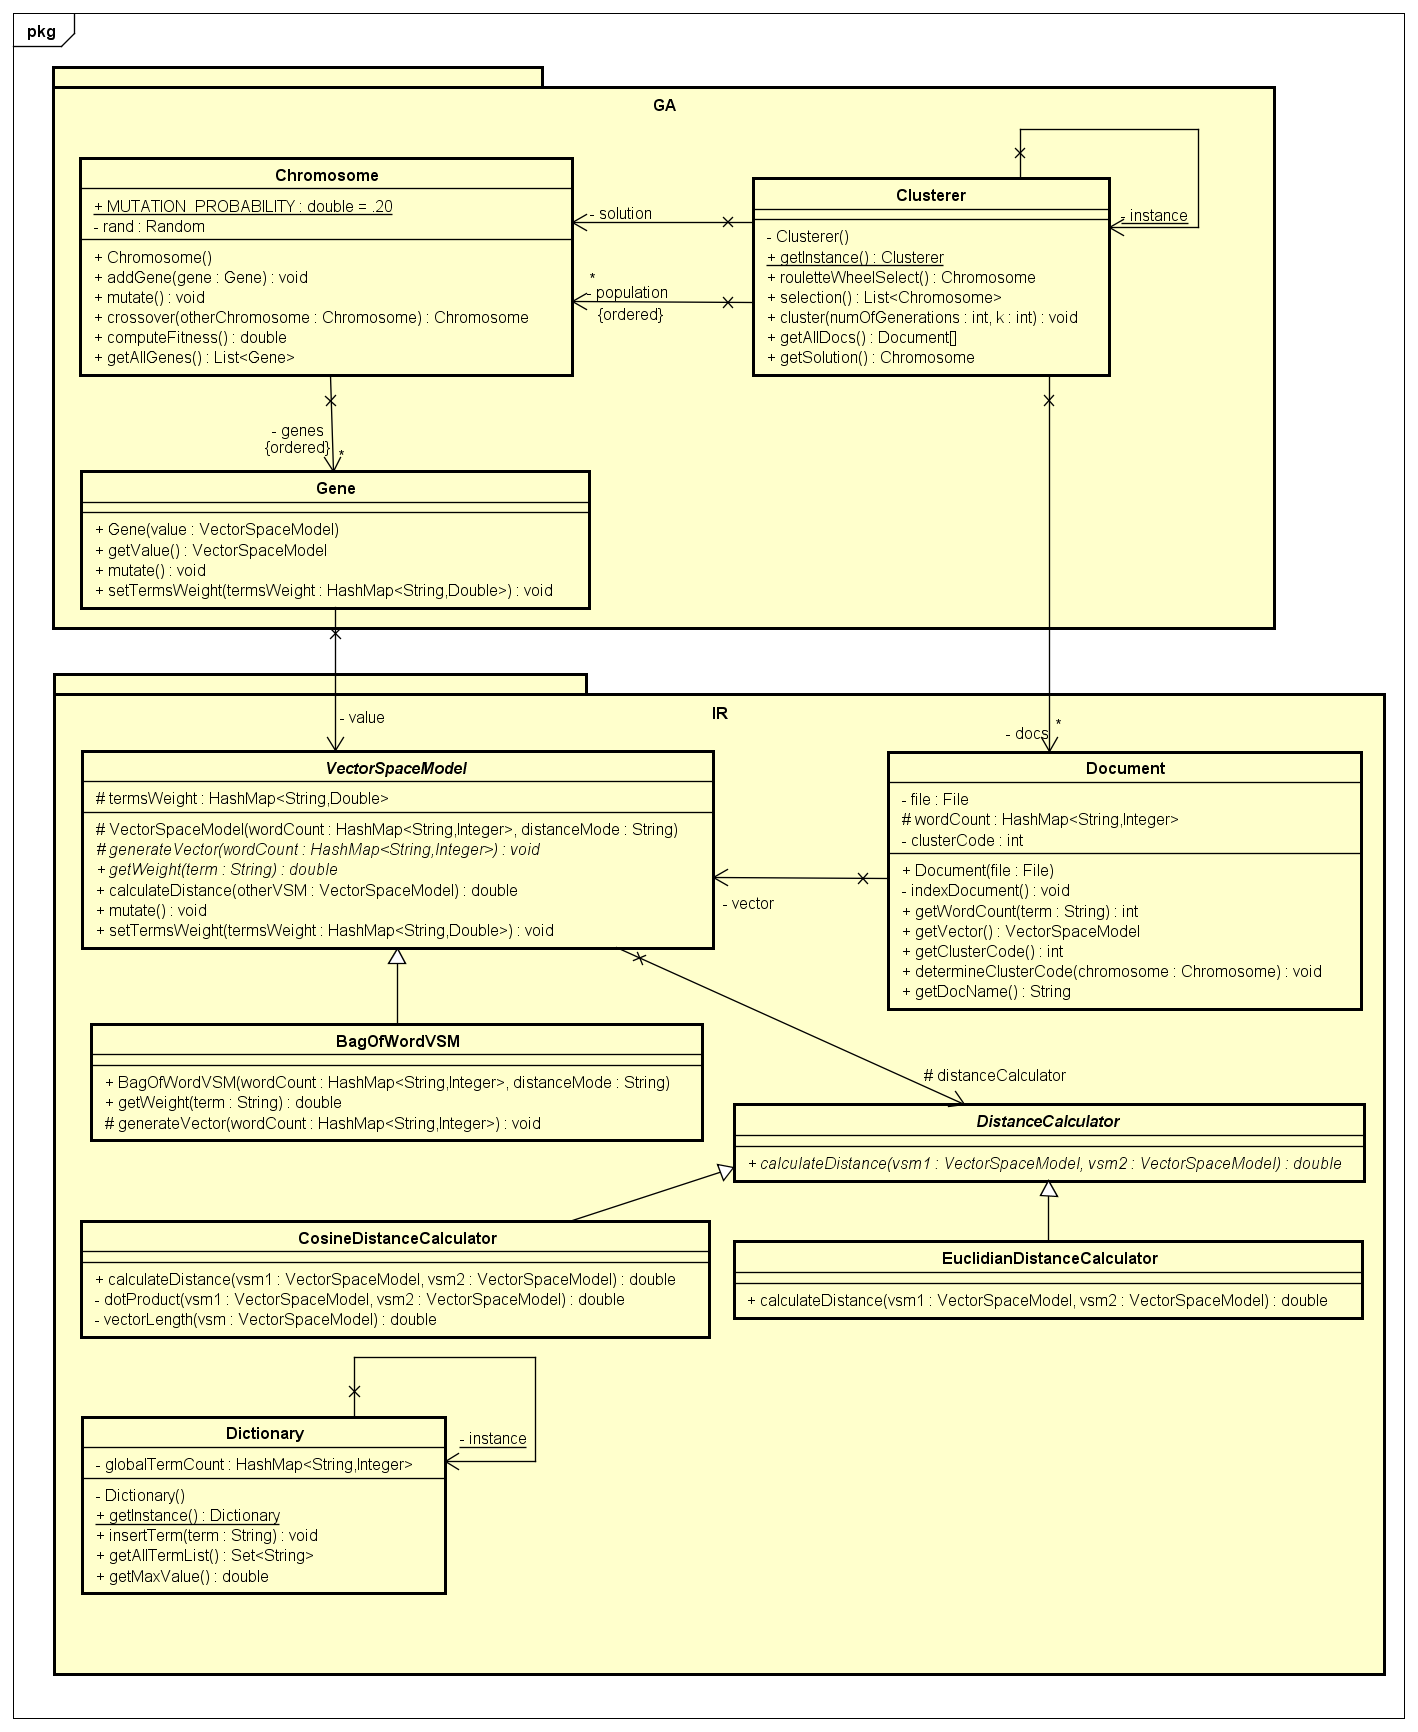
\includegraphics[width=\textwidth]{DiagramKelas}
%		\caption{\textit{Diagram Kelas}}
%		\label{fig:diagramkelas}
%	\end{center}
%\end{figure}